\part{Introduction}
\section{Preface}
Thanks to the rapid development of experimental techniques at the cellular level, over the last century there was a tremendous progress in the fields of human physiology, immunology and therapeutics. The breakthrough discoveries were based mainly on the analysis of biochemistry (either intercellular or intracellular molecular pathways).
Mechanical properties of investigated objects were often either completely neglected, or strongly underestimated. However, all living cells are exposed to the action of external forces: fluid-mediated (eg. blood flow) or structure-mediated (eg. body weight strain in bones). The process of converting external mechanical stimuli into biochemical signals (and in turn into physiological responses) is called mechanotransduction. 
\newline 
The most appealing discovery, which evidences for the importance of mechanical properties, refers to the fate of stem cells. In 2006 Engler \emph{et al.} identified a new factor capable to regulate the fate of stem cells: the elasticity of the microenvironment (matrix). Namely, by changing the elastic properties of the substrate, stem cells could be directed towards muscle, bone or even neuronal lineages \cite{Even-Ram2006}. On the grounds of the recent discoveries, the new field of science have emerged: \emph{mechanobiology}. It is targeted to study the mechanotransduction processes at the level of tissues and cells, and the way it influences the development, physiology and diseases.
One may wonder what is the range of forces capable to elicit a cellular response. It is reasonable to assume, that the effect of force should exceed the energy of thermal fluctuations. At $37\degree C$ the thermal energy, $kT$, is about $4\;pN\cdot nm$. Considering the conformational changes in peptide-based molecular transducers have a characteristic length scale within the range of $1 - 10\;nm$, then it would correspond to the force of $0.4-4\;pN$. Interestingly, Finner \emph{et al.} (1994) have estimated, that a single myosin molecule, which drives contractility action and thus can induce cell signaling, is capable to produce a force $3-4\;pN$ \cite{Silberberg2008}. Therefore, it turns out that mechanotransduction is induced by forces only slightly higher than thermal fluctuations, \emph{i.e.} within the range of $10^0-10^1$ piconewtons. Obviously, the sensitivity and concentration of force transducers strongly depends on the type of cell and its location in human body.
\newline

The endothelium is formed by the monolayer of cells lining the lumen of all blood vessels in human body. \Glspl{EC} serve as a barrier between blood and the rest of the system. Thus, their physiology is affected by numerous biochemical factors. The dysfunction of endothelium contributes to the development of numerous systemic civilization-wide diseases, \emph{inter alia} hypertension, atherosclerosis and diabetes. Therefore, a deep understanding of its functioning is one of the main interest in terms of the development of proper treatments. The vascular system is a highly dynamic structure, with component-rich blood constantly circulating in the pace of heart beats, which is followed by vessel vasodynamics. Moreover, it provides highly versatile environments -- human circulatory system is over 100 000 000 meters long and the luminal diameter varies from several centimeters (\emph{eg.} aorta) to submilimeter values (mirovessels) \cite{Loe2004, Fu2013}. Therefore, a great input to cardiovascular physiology is provided by mechanobiology of endothelium, which in turn may be considered in terms of two classes: cell mechanics and external mechanical stimuli \cite{Fels2014}. The extracellular stimulation is exerted by the cell-cell contacts and the blood flow (shear stress, circumferential stretch and hydrostatic pressure). Complementary, endothelial (nano)mechanics is understood in terms of mechanical properties of cellular structures and their variations triggered either by intracellular processes or external stimuli. Considering the importance of endothelial physiology for the homeostasis of human body and the particular role that is played by \glspl{EC} nanomechanics, these type of cells became a primary focus in the presented work.

Only recently, mechanical properties of endothelial cellular structures were proven to be in correlation with intracellular biochemical processes. The studies presented in literature mostly relate cortical elasticity variations to the changes of selected biochemical factor. 
Attempts employing various experimental techniques have been made, involving optical tweezers \cite{Wang2006, Hayakawa2008}, magnetic bead pulling/twisting \cite{Bausch2001, Zeng2010} and pipette aspiration \cite{Sato1987, Zeng2011}. 
However, the most prominent advances in this area have been made using \gls{AFM}. The group of Oberleithner (University of M\"{u}nster, Germany) became a leader in studying endothelial nanomechanics. Using nanoindentation spectroscopy with an \gls{AFM} tip, they have connected elasticity changes with aldosterone treatment \cite{Oberleithner2005}, sodium \cite{Oberleithner2007a} and potassium \cite{Oberleithner2009} concentration, \gls{NO} production \cite{Fels2010_trois}, C-reactive protein \cite{Kusche-Vihrog2011} and \gls{ENaC} activity \cite{Kusche-Vihrog2008}. Using the same technique, our group have described the alterations of \glspl{EC} mechanical properties during the development of inflammatory state triggered by \gls{TNF} \cite{Szczygiel2011}, as well as during the anti-inflammatory action of 1-methylonicotinamid chloride \cite{Kolodziejczyk2013}. Moreover, we have discovered the stiffness memory of \glspl{EC} in response to chronic hyperglycemia \cite{Targosz-Korecka2013}. 
The presented \gls{AFM}-based investigations considered the \gls{AFM} probe-cell mechanical interaction in terms of simple elastic (Hertzian) deformation. Thus, the \gls{EC} mechanical properties were effectively determined by elasticity of cell cortex (mainly cortical actin skeleton). As there exist numerous cell structures relevant in terms of nanomechanics (see section \ref{sec:cellular_structures}), lately this simplified approach became a matter of discussion. As a result, last year two papers presenting either only mechanical properties of \gls{eGC} \cite{Wiesinger2013} or \gls{eGC} together with cortical elasticity has been published. However, the presented methodology is still to be improved in order to obtain objective, unbiased results.

The presented dissertation focuses on the development of experimental protocols and data analysis procedures targeted to differentiate nanomechanical properties of individual structures in \glspl{EC}. The study was aimed at the in vitro cultured \glspl{EC} whose mechanics has been assessed basing on the character of interaction during nanoindentation with a tip of \gls{AFM}. The work is organized in the following way. Firstly, the models of interactions occuring during cell indentation with a probe will be introduced. Next, the nanoindentation data are analysed separately during probe approach, relaxation (pause segment) and retraction. Each of these segments is used to resolve information about individual cellular structures, namely \gls{eGC}, cell membrane, cell cortex and bulk. In addition, a tip-induced mechanotransduction effect is presented in section XX. Lastly, section XX describes the research, where solid-state \gls{AFM} probe has been replaced by a living \gls{EC}, which then was used to probe cell-cell interaction. The proposed experimental methodology provides solid foundations to use alterations in cell structures nanomechanics as a sensitive bioindicator of the physiological state of endothelium. 


This work was supported by the European Union from the resources of the European Regional Development Fund under the Innovative Economy Programme (grant coordinated by JCET-UJ, No POIG.01.01.02-00- 69/09). Part of this project (tip-induced mechanotransduction) has been also supported by the grant of the Polish Ministry of Science and Higher Education number 7150/E-338/M/2013.


\section{Cellular structures determining mechanical properties of cells}\label{sec:cellular_structures}
Animal cell is a complex living biological machinery containing nucleus and other membrane-bound organelles (mitochondria, Golgi aparatus etc.) suspended in cytosol. The presented description will apply to \gls{EC}, however a significant part of the facts hold for other human cell types. \Glspl{EC} form a tight monolayer on the luminal part of vessels, which permeability is mostly gated by those cells. Cells are highly sensitive to deformation. In the first approximation, they may be considered as a membrane-limited container filled with incompressible fluid (cytosol). Therefore, the application of an external force results in mechanical deformation of the surface, which causes the displacement of the fluid. In order to counteract the susceptibility to such stimuli and stabilize the shape, \glspl{EC} have developed a multilevel system of cytoskeletal structures composed of three polymers, namely: F-actin, intermediate filaments and tubulin. Moreover, the cellular membrane is decorated with glycan-rich brush referred to as \gls{eGC}.


\begin{figure}[tb]%H
\centering
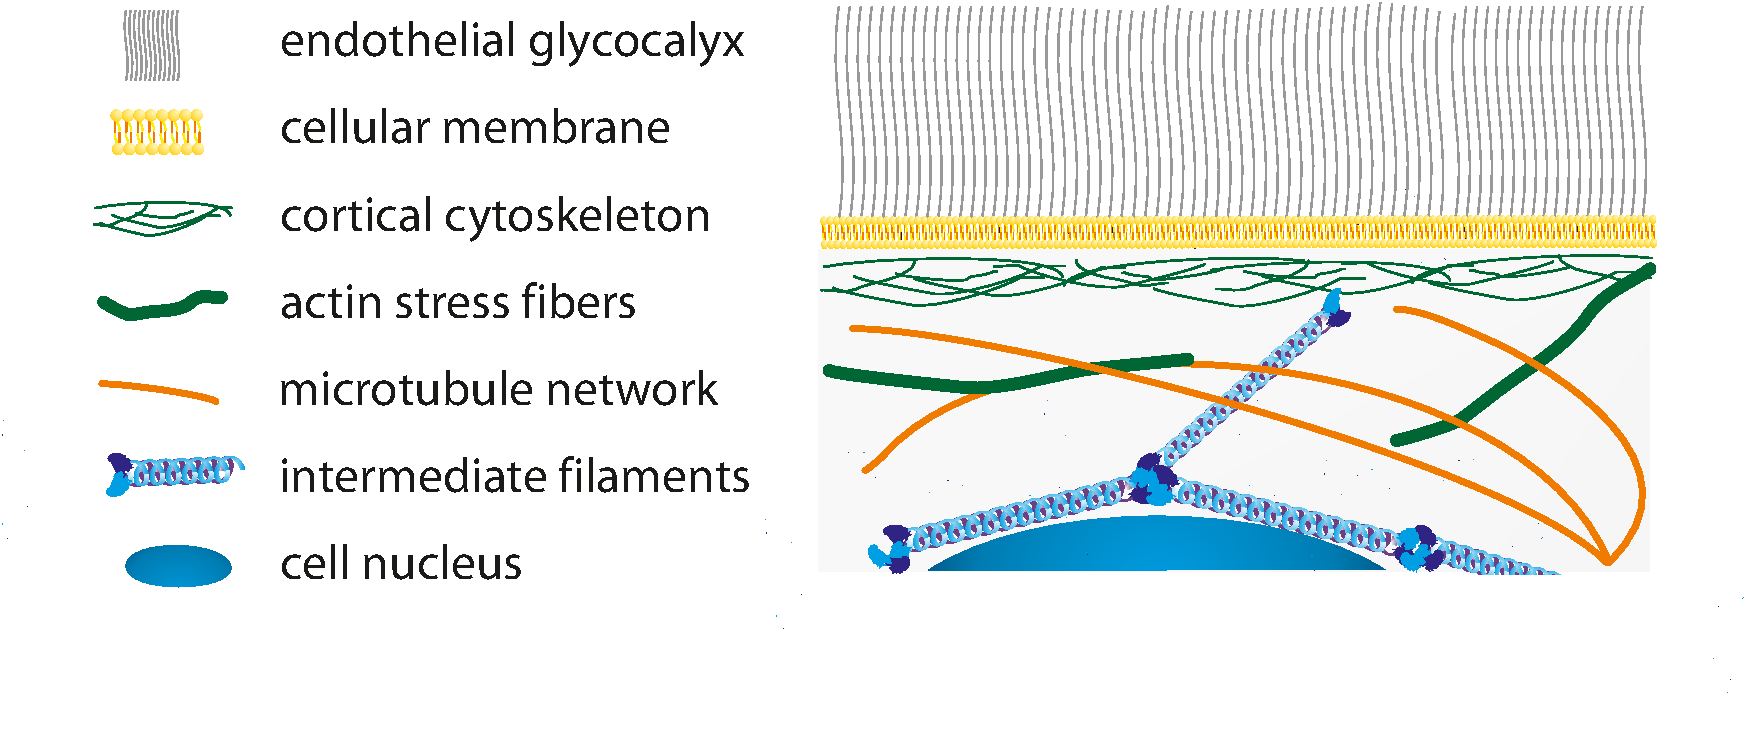
\includegraphics[width=0.9\textwidth]{schemat_komorki.pdf}
\caption[Scheme presenting cellular structures determining mechanical properties of \gls{EC}.]{The drawing presents cell components, which determine mechanical properties of \gls{EC}. The details of the structure composition and functions are presented in the text. Please note the elements are not in scale.}
\label{fig:intro:cell_structure}
\end{figure}
The schematic drawing of cell presenting the composition of cellular structures meaningful in terms of cellular mechanics is presented in Figure \ref{fig:intro:cell_structure}. Below, we will provide a brief description of each structure and its functions.
\begin{description}
\item[endothelial glycocalyx] It decorates the luminal surface of \glspl{EC} monolayer. \gls{eGC} is composed of various proteoglycans, glycosaminoglycans and plasma proteins. Transmembrane syndecans provide a direct binding of \gls{eGC} to cortical actin cytoskeleton. The components are organized in small domains ($\approx 100\;nm$), each having quasi-periodic ultrastructure with fiber diameter $\approx 10\;nm$ and spacing $\approx 20\;nm$ (characteristic dimensions calculated for frog microvascular endothelium by Squire \emph{et. al}) \cite{Squire2001}. The thickness of \gls{eGC} varies from $100\;nm$ in microvessels to over $2\;\mu m$ in large vessels (eg. aorta) \cite{Fu2013,Wiesinger2013}. \gls{eGC} is a dynamic structure, particularly sensitive to ionic homeostatis. In the absence of extracellular fluid it collapses (eg. during cell drying). Hence, the initial attempts to visualize \gls{eGC} using electron microscopy ($20\;nm$ -- Luft 1966, $40\;nm$ -- Sims \emph{et al.} 1994, $50\;nm$ -- Rostgaard \emph{et al.} 1997) severely underestimated its thickness. As a consequence, the role of \gls{eGC} also has been partialy neglected, as it was considered to be lower than some of cellular membrane channels. Only after introducing \gls{eGC} \emph{in vivo} (like intravital microscopy \cite{Gao2010}) and \emph{in vitro} (like \gls{AFM} \cite{Oberleithner2011}) imaging techniques, \gls{eGC} thickness has been correctly estimated. It was also shown, that blood flow stimulates \gls{eGC} development.
\gls{eGC} presents a negative charge, which provides repulsion of blood elements and facilitates blood flow \cite{Schnitzer1988}. Moreover, \gls{eGC} serves as mechanosensor. The signals can be transduced either directly by \gls{eGC} components (eg. through caveolae-linked glypicans containing hialuronic acid) or in cell cortex (presumably by transmembrane connections to actin structures) \cite{Davies1995}. The location of \gls{eGC} at vessel lumen makes it the first barrier for blood elements interacting with vessel wall. Thus, it takes part in the regulation of adhesion, transmigration and invagination processes.
\item[cell membrane] This structure is formed by phospholipid bilayer separating the cell interior from the external environment. Numerous membrane complexes are embedded there, either passing through the membrane or being bound at the intra or extra cellular side. These are proteins (up to $50\%$ of membrane weight) that mostly provide membrane-specific functions, eg. ion channels (transport proteins), integral proteins or peripheral proteins \cite{Cooper2000}. There are also structures formed by cholesterol (lipid rafts). Besides protecting cell content from the surrounding environment, membrane facilitates numerous cellular processes such as cell signaling, adhesion, ion conductivity and molecular transit. What is important for cell mechanics, it serves as anchoring surface for \gls{eGC} and intracellular cytoskeleton. The elasticity of cell membrane is most often defined basing on fluid mosaic model, proposed by Singer and Nicolson in 1962, where lipid molecules are assumed to move freely \cite{Singer1972}. 
\item[actin cytoskeleton] Actin protein can be present either in a monomeric globular form (G-actin) or it can form a linear double helix polymer ($7\;nm$ diameter) referred to as F-actin and it constitutes about $5-15\%$ of the total protein mass in \gls{EC} \cite{Patterson2001}. This is a highly dynamic structure -- it undergoes cell-regulated transition between G-actin and F-actin form referred to as polymerization and depolymerization process in a minute time scale \cite{Prasain2009}. There are two distinct cytoskeletal structures formed by actin in \gls{EC}: cortical cytoskeleton and stress fibres. The cortical cytoskeleton, formed by cross-linked F-actin microfilaments, lies just below the cell membrane, stabilizes it and is utilized for mobility. The Young modulus of single microfilament is around $2\;GPa$ \cite{Kojima1994}. Stress fibers are formed by microfilaments grouped into $200-500\;nm$ diameter thick bundles, together with myosin and other proteins that bind to actin \cite{Satcher1996}. They are responsible for cell stability and force generation. This is also the main structure that reinforces the cell during exposition to sheer stress during blood flow. Together with actin-binding proteins, like \gls{eNOS}, actin cytoskeleton serves as a sensitive sensor and transducer of mechanosignals \cite{Shao2014}. 
\item[microtubule network] Microtubule is a long (tens of microns) hollowed cylinder (outer diameter $24\;nm$, inner diameter $12\;nm$ composed of 13 protofilaments (polymerized linear tubulin chains). Microtubules are nucleated and governed by dedicated organelles, like centrosom. Apart from providing mechanical support and resisting cell contraction, microtubules serve as tracks dedicated for intracellular transport (provided by motor proteins). They are also involved in cell division process, when they form mitotic spindle. Microtubules are significantly more rigid than microfilaments, with Young modulus around $17\; GPa$ \cite{Kis2008}.
\item[intermediate filaments] This linear structures, which span across cytoplasm, are formed by two anti-parallel helices of various peptides (vimentin, keratins and lamins, with the first being most abundant in \gls{EC}). The average diameter is $10\;nm$, which locates this structure between actin microfilaments and microtubules (thus the name: intermediate). Thanks to the alpha-helix organization, the polymer forming intermediate filaments can be stretched several times its initial length, when transition to beta-sheets organization occurs. Basing on the span of stretch, various intracellular signals are transduced by those structures, thus intermediate filaments are considered to be stretch mechanosensors \cite{Qin2009}. The elastic modulus of those structures was reported to be in a range of megapascals \cite{Herrmann2007}. In \gls{EC}, intermediate filaments work synergistically with other compounds of cytoskeleton, and are mostly responsible for bearing tension.
\item[cell nucleus] Most of the cell's genetic material is stored inside nucleus. Therefore, this membrane-enclosed organelle is filled with DNA mixed with various complex proteins. The nucleus was show to be 10 times stiffer than the surrounding cytoplasm \cite{Martins2012}. It is supported and linked to all aforementioned cytoskeletal components through various peptides. Only recently Swift \emph{et al.} have proposed, that cell nucleus may act as intracellular \emph{mechanostat}, that not only senses and transduces mechanical signals mediated by other cytoskeletal structures, but also adjusts its own elastic properties to the extracellular environment \cite{Swift2013}.
\end{description}

\section{Materials and equipment}
All experiments have been performed in the Department of Nanostructures and Nanotechnology at the Institute of Physics, Jagiellonian University in Krakow, excluding the Section \ref{sec:tip-induced_mechanotransduction}, which was partially conducted at the Institute of Physiology II, University of M\"{u}nster, Germany.
\subsection{Cell culture}
Unless stated otherwise, the presented experiments were conducted on EA.hy926 endothelial cells. This is a relatively stable, well established cell line derived from \glspl{HUVEC} immortalized by fusing with human lung carcinoma cell line A549 by Edgell \emph{et al.} in 1983 \cite{Edgell1983}. Cell culture was kindly maintained by Marta Targosz-Korecka and Katarzyna Ma\l{}ek from our group. Briefly, cells were cultured in Dulbecco's Modified Eagle's Medium (DMEM, Cat. No. 30-2002, Invitrogen) supplemented by $2\%$ HAT supplement (Cat. No. 21060-017, Invitrogen), $10\%$ fetal bovine serum (FBS, Cat. No. 10082-147, Invitrogen). Cells were maintained in 
$75\;cm^2$ culture flasks placed in an incubator-controlled atmosphere
($37\degree C$, fully humidified with $5\%\ CO_2$) to reach confluence and then they were passaged. After trypsinization, cells were centrifuged and resuspended in medium. Part of the solution was seeded on glass slides placed in multiwell plates and the rest was introduced to culture flask to maintain the culture. The cells placed on the glass slides were then incubated for 48h in the presence of $10\%$ FBS and then taken for \gls{AFM} measurements. The details of culturing protocol are described in our papers \cite{Szczygiel2011, Targosz-Korecka2013}.
\subsection{Fluorescence microscopy}
\todo{Opisać fluorescencje w Muenster, jesli zamieszcze jakies zdjecia}

